\documentclass[12pt, a4paper]{article}

\usepackage[margin=2.5cm, top=3cm, bottom=3cm]{geometry}
\emergencystretch=3em
\tolerance=1200
\usepackage[table]{xcolor}
\usepackage{amsmath}
\usepackage{amssymb}
\usepackage{booktabs}
\usepackage{array}
\usepackage{tabularx}
\usepackage{graphicx}
\usepackage{hyperref}
\usepackage{fancyhdr}
\usepackage{titlesec}
\usepackage{parskip}
\usepackage{enumitem}
\usepackage[letterspace=150]{microtype}
\usepackage{mdframed}
\usepackage{lmodern}
\usepackage{fontenc}
\usepackage{inputenc}
\usepackage{caption}
\usepackage{subcaption}
\usepackage{float}
\usepackage{multirow}
\usepackage{longtable}
\usepackage{tcolorbox}
\tcbuselibrary{skins, breakable}

\definecolor{ehaBlue}{RGB}{0, 84, 142}
\definecolor{ehaLightBlue}{RGB}{224, 237, 248}
\definecolor{ehaGrey}{RGB}{245, 245, 245}
\definecolor{ehaAccent}{RGB}{0, 153, 118}
\definecolor{ehaRed}{RGB}{192, 57, 43}
\definecolor{ehaAmber}{RGB}{230, 126, 34}
\definecolor{tableHead}{RGB}{0, 84, 142}
\definecolor{tableAlt}{RGB}{240, 248, 255}
\definecolor{resolvedGreen}{RGB}{39, 174, 96}

\hypersetup{
  colorlinks=true, linkcolor=ehaBlue, urlcolor=ehaBlue,
  pdftitle={TRACE Evaluation Report --- SARMAAN LC Dashboard (August 2026)},
  pdfauthor={eHealth Africa},
}

\pagestyle{fancy}
\fancyhf{}
\fancyhead[L]{\small\textcolor{ehaBlue}{\textbf{eHealth Africa $\mid$ SARMAAN LC Dashboard --- TRACE Evaluation}}}
\fancyhead[R]{\small\textcolor{gray}{August 2026}}
\fancyfoot[C]{\small\textcolor{gray}{\thepage}}
\renewcommand{\headrulewidth}{0.4pt}
\renewcommand{\headrule}{\hbox to\headwidth{\color{ehaBlue}\leaders\hrule height\headrulewidth\hfill}}
\setlength{\headheight}{25.4pt}

\titleformat{\section}{\large\bfseries\color{ehaBlue}}{\thesection.}{0.6em}{}[\titlerule]
\titleformat{\subsection}{\normalsize\bfseries\color{ehaBlue!80!black}}{\thesubsection}{0.6em}{}
\titleformat{\subsubsection}{\small\bfseries\color{ehaBlue!60!black}}{\thesubsubsection}{0.6em}{}
\titlespacing*{\section}{0pt}{1.6em}{0.7em}
\titlespacing*{\subsection}{0pt}{1.1em}{0.4em}
\titlespacing*{\subsubsection}{0pt}{0.9em}{0.3em}

\mdfdefinestyle{keybox}{
  backgroundcolor=ehaLightBlue, linecolor=ehaBlue, linewidth=1pt,
  innerleftmargin=12pt, innerrightmargin=12pt,
  innertopmargin=10pt, innerbottommargin=10pt, roundcorner=4pt,
}
\mdfdefinestyle{warnbox}{
  backgroundcolor=ehaAmber!12, linecolor=ehaAmber, linewidth=1.5pt,
  topline=false, rightline=false, bottomline=false,
  innerleftmargin=12pt, innerrightmargin=12pt,
  innertopmargin=8pt, innerbottommargin=8pt,
}
\mdfdefinestyle{alertbox}{
  backgroundcolor=ehaRed!8, linecolor=ehaRed, linewidth=1.5pt,
  topline=false, rightline=false, bottomline=false,
  innerleftmargin=12pt, innerrightmargin=12pt,
  innertopmargin=8pt, innerbottommargin=8pt,
}
\mdfdefinestyle{greenbox}{
  backgroundcolor=ehaAccent!10, linecolor=ehaAccent, linewidth=1.5pt,
  topline=false, rightline=false, bottomline=false,
  innerleftmargin=12pt, innerrightmargin=12pt,
  innertopmargin=8pt, innerbottommargin=8pt,
}
\mdfdefinestyle{mitigbox}{
  backgroundcolor=ehaBlue!6, linecolor=ehaBlue, linewidth=1.5pt,
  topline=false, rightline=false, bottomline=false,
  innerleftmargin=12pt, innerrightmargin=12pt,
  innertopmargin=8pt, innerbottommargin=8pt,
}

\newcolumntype{L}[1]{>{\raggedright\arraybackslash}p{#1}}
\newcolumntype{C}[1]{>{\centering\arraybackslash}p{#1}}
\newcolumntype{R}[1]{>{\raggedleft\arraybackslash}p{#1}}

\captionsetup{font=small, labelfont={bf,color=ehaBlue}, labelsep=period,
              skip=6pt, width=0.95\textwidth}

\newcounter{finding}
\newcommand{\finding}[1]{%
  \stepcounter{finding}%
  \begin{mdframed}[style=greenbox]
  \textbf{Finding \thefinding:} #1
  \end{mdframed}%
}
\newcounter{issue}
\newcommand{\issuelabel}[2]{%
  \stepcounter{issue}%
  \begin{mdframed}[style=alertbox]
  \textbf{Issue \theissue\ [\textcolor{ehaRed}{#1}]:} #2
  \end{mdframed}%
}
\newcommand{\mitigation}[1]{%
  \begin{mdframed}[style=mitigbox]
  \textbf{\textcolor{ehaBlue}{Mitigation:}} #1
  \end{mdframed}%
}

\begin{document}

% ════════════════════════════════════════════════════════════════════════════════
%  TITLE PAGE
% ════════════════════════════════════════════════════════════════════════════════
\begin{titlepage}
  \pagecolor{ehaBlue}\color{white}
  \vspace*{1.8cm}

  {\fontsize{10}{12}\selectfont\MakeUppercase{\textls[100]{TRACE Evaluation Report}}}\\[0.5em]
  {\fontsize{26}{32}\selectfont\bfseries TRACE Evaluation\\[0.3em]
   SARMAAN LC Dashboard}\\[1.2em]
  \textcolor{ehaAccent}{\rule{6cm}{2pt}}\\[1.2em]

  {\large SARMAAN LGA Coordinator (LC) Dashboard}\\[0.4em]
  {\normalsize eHealth Africa $\cdot$ SARMAAN / Kano AMR}\\[2.5cm]

  \begin{tabular}{@{}ll}
    \textbf{Document Version}  & 1.0 \\[0.4em]
    \textbf{Date}              & August 2026 \\[0.4em]
    \textbf{Repository}        & sarmaan\_lc\_dashboard \\[0.4em]
    \textbf{Branch}            & \texttt{feature/trace-evaluation} \\[0.4em]
    \textbf{Commit Evaluated}  & \texttt{484e2d9} \\[0.4em]
    \textbf{Framework}         & TRACE (Technical / Real-world / Adaptive / Outcomes / Economic) \\[0.4em]
    \textbf{Evaluated By}      & Joshua Ogundairo (with Claude Code) \\[0.4em]
    \textbf{Overall Score}     & \textbf{4.59 / 10} \\[0.4em]
    \textbf{Status}            & Final \\
  \end{tabular}

  \vfill
  {\small\textcolor{white!70!ehaBlue}
    {This report documents the design, scope, and results of a TRACE
     evaluation of The SARMAAN LGA Coordinator (LC) Dashboard -- a zero-infrastructure static site plus an hourly GitHub Actions KoboToolbox data pipeline -- as a software product, including its actual current live operational state, not only its designed intent. It
     records what was scored, on what evidence, what was found, and what
     remains open for follow-up.}}
\end{titlepage}
\pagecolor{white}\color{black}

% ════════════════════════════════════════════════════════════════════════════════
%  TABLE OF CONTENTS
% ════════════════════════════════════════════════════════════════════════════════
\tableofcontents
\clearpage

% ════════════════════════════════════════════════════════════════════════════════
%  1. EXECUTIVE SUMMARY
% ════════════════════════════════════════════════════════════════════════════════
\section{Executive Summary}

This report applies the TRACE Evaluation Framework to the SARMAAN LGA Coordinator (LC) Dashboard --- a deliberately zero-infrastructure static site paired with an hourly GitHub Actions pipeline that pulls field-submission data from KoboToolbox --- as it stands on \texttt{main} (commit \texttt{484e2d9}). TRACE scores a complex intervention across five weighted pillars --- Technical, Real-world, Adaptive, Outcomes, Economic --- looking at the whole trajectory (the \emph{how}) alongside the final result (the \emph{what}), not a single-point metric.

\textbf{This evaluation surfaced a live, currently-ongoing operational failure}, not just a static code review: the repository's own automated data pipeline has failed 100 out of its last 100 recorded runs (verified via \texttt{gh run list}), with the specific error \texttt{KOBO\_TOKEN environment variable not set} (verified via \texttt{gh run view --log-failed}), and GitHub Pages is not even enabled for this repository (confirmed via the GitHub API). The scores below reflect the platform's \emph{actual current state}, not only its designed intent --- this is a deliberate and, per this report's framing, necessary departure from evaluating code quality in isolation.

\begin{mdframed}[style=keybox]
\textbf{Key Numbers at a Glance}
\begin{itemize}[noitemsep, topsep=2pt]
  \item \textbf{Overall TRACE score: 4.59 / 10} across 5 pillars and 15 criteria --- the lowest score in this evaluation batch, driven almost entirely by a currently-broken production deployment rather than by code quality
  \item \textbf{The system's one automated job has a 0\% success rate}: 100 of the last 100 \texttt{Fetch KoboToolbox Data} workflow runs have failed with \texttt{KOBO\_TOKEN environment variable not set} --- a one-line configuration fix (adding the missing GitHub Actions secret), not a code defect
  \item \textbf{Data has been frozen for over 5 weeks}: \texttt{data.json} is stamped \texttt{fetched\_at: 2026-07-07 01:05 WAT}, more than five weeks stale as of this evaluation (2026-08-11)
  \item \textbf{GitHub Pages is not enabled for this repository} (confirmed via \texttt{gh api repos/.../pages} returning 404) --- there is currently no live URL serving this dashboard at all, despite the README's detailed deployment guide
  \item \textbf{Strongest pillar: Economic (6.33 / 10)} --- the underlying `zero-infrastructure' architecture (no server, no database, no hosting bill) is genuinely well-designed and remains sound even while the pipeline is down
\end{itemize}
\end{mdframed}

\clearpage

% ════════════════════════════════════════════════════════════════════════════════
%  2. FRAMEWORK AND METHODOLOGY
% ════════════════════════════════════════════════════════════════════════════════
\section{Framework and Methodology}

TRACE evaluates an intervention across five weighted pillars. Each pillar
is scored as the mean of its own criteria (each criterion scored 0--10
against cited evidence); the overall score is the weight-weighted mean of
the five pillar scores, also on a 0--10 scale. A criterion score without a
written justification is rejected by the scoring tool --- every number in
this report traces back to a specific, citable piece of evidence.

\begin{table}[H]
\centering
\caption{TRACE pillars and weights}
\label{tab:pillars}
\small
\rowcolors{2}{tableAlt}{white}
\begin{tabularx}{\linewidth}{L{2.6cm} C{1.6cm} X}
\toprule
\rowcolor{tableHead}
\textcolor{white}{\textbf{Pillar}} &
\textcolor{white}{\textbf{Weight}} &
\textcolor{white}{\textbf{What it measures}} \\
\midrule
Technical & 20\% & Functional, structural, and foundational robustness of the intervention. \\
Real-world & 25\% & Performance in authentic, noisy environments rather than controlled, ideal settings. \\
Adaptive & 20\% & The capacity to learn, change, and improve based on feedback. \\
Outcomes & 25\% & The final results, evaluating whether the intended goals were achieved effectively. \\
Economic & 10\% & The financial viability and efficiency of the intervention. \\
\bottomrule
\end{tabularx}
\end{table}

\begin{mdframed}[style=mitigbox]
\textbf{Scoring scale:} 0--10 per criterion. \textbf{$\geq$7.0}: strong,
evidenced, no material gap. \textbf{5.0--6.9}: adequate, with a specific,
named gap. \textbf{$<$5.0}: weak --- an open risk or unmeasured area that
should be treated as a priority action.
\end{mdframed}

\subsection*{Criteria by Pillar}

\subsection{Technical (20\%)}
Functional, structural, and foundational robustness of the intervention.
\begin{itemize}[noitemsep]
  \item \textbf{System Performance} --- The technical ability to navigate information, use tools, and generate accurate results.
  \item \textbf{Evidence Grounding} --- Outputs are supported by factual evidence — preventing hallucinated or unreliable reasoning.
  \item \textbf{Process Efficiency} --- The ability to achieve goals with minimal, necessary actions rather than redundant, wasteful ones.
\end{itemize}

\subsection{Real-world (25\%)}
Performance in authentic, noisy environments rather than controlled, ideal settings.
\begin{itemize}[noitemsep]
  \item \textbf{Realism \& Robustness} --- How well the system performs against unexpected challenges, information traps, and messy/incorrect data.
  \item \textbf{Context Applicability} --- How the tool adapts to diverse, complex organizational or social settings.
  \item \textbf{Safety \& Reliability} --- Whether, in practice, the system behaves in a safe and controllable manner.
\end{itemize}

\subsection{Adaptive (20\%)}
The capacity to learn, change, and improve based on feedback.
\begin{itemize}[noitemsep]
  \item \textbf{Self-Correction} --- Ability to recover from errors (recovery latency).
  \item \textbf{Iterative Design} --- A 'living document' approach where methodologies are updated based on ongoing monitoring.
  \item \textbf{Feedback Loops} --- Utilizing feedback — natural language feedback or performance scores — to refine strategies dynamically.
\end{itemize}

\subsection{Outcomes (25\%)}
The final results, evaluating whether the intended goals were achieved effectively.
\begin{itemize}[noitemsep]
  \item \textbf{Final Success} --- The accuracy of the final answer, product, or policy outcome.
  \item \textbf{Impact Analysis} --- The difference the intervention made — e.g. reducing cost/risk, improving productivity, changing behavior.
  \item \textbf{Process-Outcome Link} --- How effectively the intermediate steps (trajectory) led to the final outcome.
\end{itemize}

\subsection{Economic (10\%)}
The financial viability and efficiency of the intervention.
\begin{itemize}[noitemsep]
  \item \textbf{Cost-Benefit Analysis} --- Whether the benefits of the intervention outweigh the costs of implementation.
  \item \textbf{Efficiency Analysis} --- How well resources are used (cost-effectiveness).
  \item \textbf{Scalability} --- Whether the solution can be scaled sustainably without prohibitive expenses.
\end{itemize}

\clearpage

% ════════════════════════════════════════════════════════════════════════════════
%  3. RESULTS
% ════════════════════════════════════════════════════════════════════════════════
\section{Results}

\subsection{Scorecard}

\begin{table}[H]
\centering
\caption{TRACE pillar scorecard}
\label{tab:scorecard}
\small
\rowcolors{2}{tableAlt}{white}
\begin{tabularx}{\linewidth}{X C{1.6cm} C{1.6cm} C{3.4cm}}
\toprule
\rowcolor{tableHead}
\textcolor{white}{\textbf{Pillar}} &
\textcolor{white}{\textbf{Weight}} &
\textcolor{white}{\textbf{Score}} &
\textcolor{white}{\textbf{Rating}} \\
\midrule
Technical & 20\% & 5.33 & \textcolor{ehaAmber}{\textbf{Adequate, with gaps}} \\
Real-world & 25\% & 5.67 & \textcolor{ehaAmber}{\textbf{Adequate, with gaps}} \\
Adaptive & 20\% & 3.00 & \textcolor{ehaRed}{\textbf{Weak}} \\
Outcomes & 25\% & 3.50 & \textcolor{ehaRed}{\textbf{Weak}} \\
Economic & 10\% & 6.33 & \textcolor{ehaAmber}{\textbf{Adequate, with gaps}} \\
\midrule
\multicolumn{2}{r}{\textbf{Overall (weighted)}} & \textbf{4.59} &
  \textcolor{ehaRed}{\textbf{Weak}} \\
\bottomrule
\end{tabularx}
\end{table}

\begin{figure}[H]
  \centering
  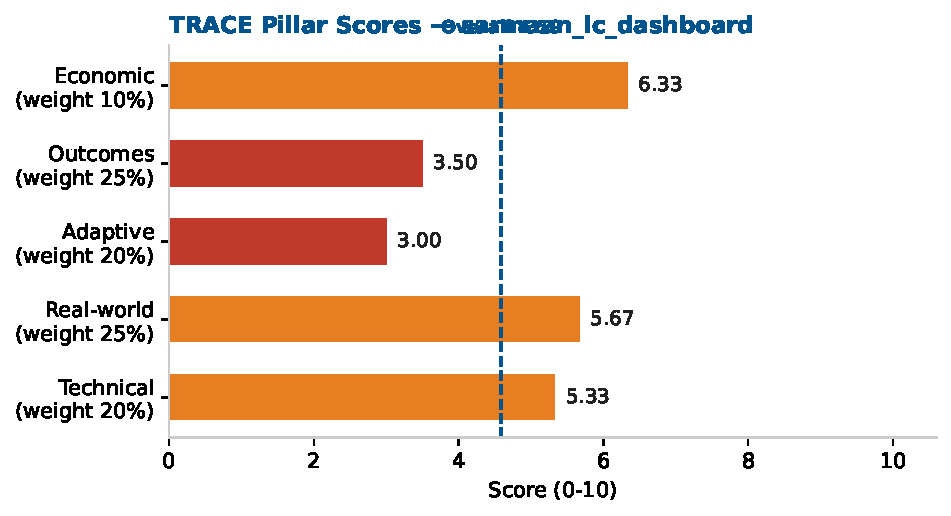
\includegraphics[width=0.92\textwidth]{figures/fig01_pillar_scorecard.pdf}
  \caption{Weighted score per pillar against the overall score (dashed line).}
  \label{fig:pillar_scorecard}
\end{figure}

\begin{figure}[H]
  \centering
  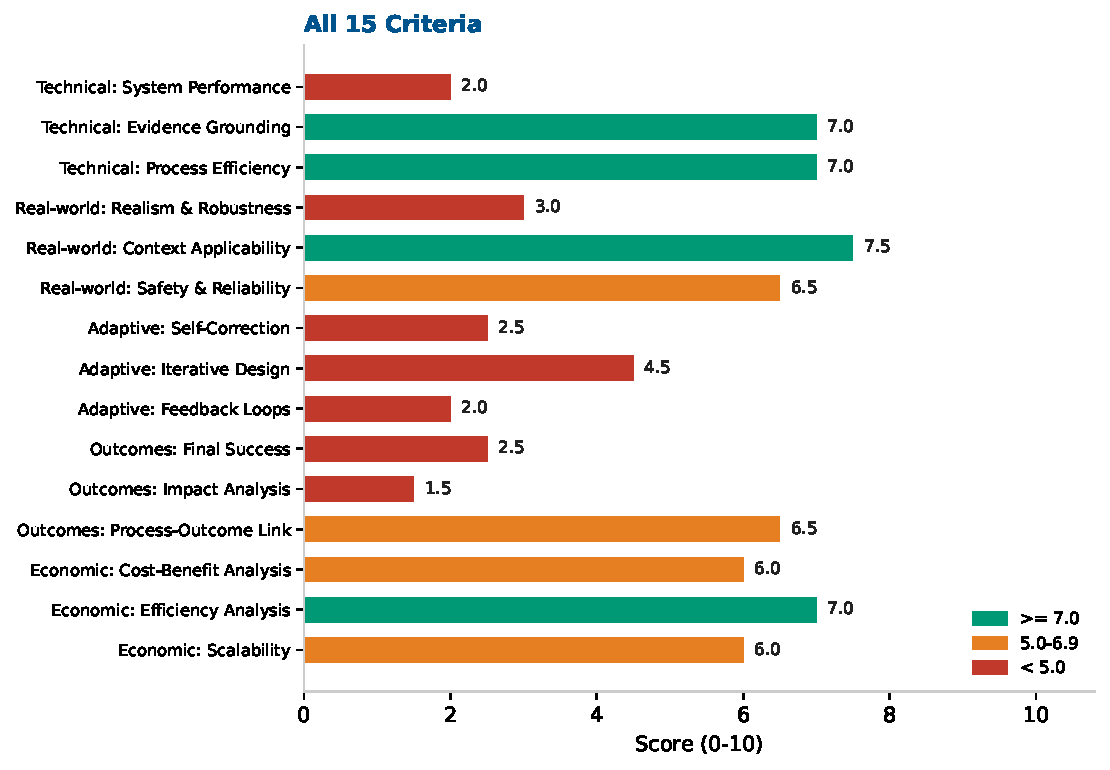
\includegraphics[width=0.95\textwidth]{figures/fig02_criterion_detail.pdf}
  \caption{All 15 individual criterion scores, color-banded by rating.}
  \label{fig:criterion_detail}
\end{figure}

\clearpage

\subsection{Criterion-Level Detail}

Each box below states the criterion's score and the specific evidence it
is grounded in. Colour follows the same scale as Table~\ref{tab:scorecard}
(green $\geq$7.0, amber 5.0--6.9, red $<$5.0).

\subsection{Technical --- 5.33 / 10}
\begin{mdframed}[style=alertbox]\textbf{System Performance --- 2.0 / 10}\\
The system's one automated job -- hourly fetch of KoboToolbox data via GitHub Actions -- has failed 100 out of the last 100 recorded runs (verified via `gh run list`), with the specific, exact error `ERROR: KOBO\_TOKEN environment variable not set` (verified via `gh run view --log-failed`). `data.json` is frozen at `fetched\_at: 2026-07-07 01:05 WAT` with 742 rows, more than five weeks stale as of this evaluation's date (2026-08-11). This is a complete, currently-ongoing operational failure of the system's entire reason for existing, not a hypothetical or historical risk.\end{mdframed}
\begin{mdframed}[style=greenbox]\textbf{Evidence Grounding --- 7.0 / 10}\\
fetch\_data.py's `clean(row)` function and its `g(row, key)` helper are compact and well-scoped, and README.md explicitly documents the exact shape and meaning of every field the frontend consumes (date, coord, lga, status, activity flags, DC roster counts, issue flags). The README's own troubleshooting guidance states the dashboard 'never mutates the file,' so any numeric mismatch a user sees is traceable directly back to the raw Kobo data -- a genuinely well-grounded, if small, data contract.\end{mdframed}
\begin{mdframed}[style=greenbox]\textbf{Process Efficiency --- 7.0 / 10}\\
Deliberately minimal-dependency design (Python 3 standard library only for the fetch script, no frontend build step, Chart.js loaded from a CDN) means there is very little to run inefficiently. Each hourly workflow run only commits when the fetched data actually changed (`git diff --cached --quiet || git commit ...`), avoiding no-op commit noise on unchanged data.\end{mdframed}

\subsection{Real-world --- 5.67 / 10}
\begin{mdframed}[style=alertbox]\textbf{Realism \& Robustness --- 3.0 / 10}\\
The one deliberate robustness feature -- a coloured freshness status dot (green/amber/red) meant to surface a fetch failure directly to end users -- is a sound design idea, but this evaluation found the system has been in the state that dot is meant to flag (fetch failed) continuously for over five weeks, and nothing beyond that in-page visual indicator (no alerting, no notification to a maintainer) surfaces the failure to anyone not actively looking at the page. The safety mechanism exists but has not, in practice, triggered a fix.\end{mdframed}
\begin{mdframed}[style=greenbox]\textbf{Context Applicability --- 7.5 / 10}\\
Purpose-built for the real role structure of the SARMAAN/Kano AMR programme: LGA Coordinators reporting daily field activity, with domain-specific fields matching how this specific programme is organized -- geofence in/out-of-LGA status with collected reasons, a Data Collector roster (present/partially present/absent), and an activity-type breakdown (training, field coordination, supervision, stakeholder engagement, problem solving/escalations) that mirrors the coordinators' actual job categories rather than a generic activity log.\end{mdframed}
\begin{mdframed}[style=warnbox]\textbf{Safety \& Reliability --- 6.5 / 10}\\
Explicit, honest security design: the Kobo API token lives only in a GitHub Actions secret and README.md confirms it 'never appears in any committed file'; `data.json` is deliberately scoped to non-PII fields with a direct instruction to 'review new fields before adding them to clean(row)'; the README is unusually candid about the public-repo tradeoff required for free GitHub Pages ('treat everything in data.json as world-readable... If you need to hide fields, either drop them in clean(row) or move to a private repo'). Held down by a real, concrete gap: the one secret this entire design depends on (`KOBO\_TOKEN`) was never actually configured on this specific repository (see System Performance), so the documented security posture and the actual configured state have drifted apart.\end{mdframed}

\subsection{Adaptive --- 3.00 / 10}
\begin{mdframed}[style=alertbox]\textbf{Self-Correction --- 2.5 / 10}\\
Only 2 real, human-authored commits exist beyond the 373 automated hourly data-refresh commits (a README expansion, and a UI/UX standards pass) -- no bug-fix commit is visible anywhere in the history. Most importantly, the one concrete defect this evaluation found (the missing `KOBO\_TOKEN` secret causing a 100\% pipeline failure rate) has been present and unaddressed for over a month despite being trivially visible on the repository's own Actions tab.\end{mdframed}
\begin{mdframed}[style=alertbox]\textbf{Iterative Design --- 4.5 / 10}\\
README.md is a genuinely well-organized, thorough living document for the code's size -- an architecture diagram, a configuration reference, a troubleshooting table, and a dedicated security-notes section. But it describes an intended steady state rather than showing evidence of active iteration: with only 2 real commits and an ongoing, unaddressed operational failure, there is little sign of this documentation (or the underlying system) being actively kept in sync with the platform's actual current state.\end{mdframed}
\begin{mdframed}[style=alertbox]\textbf{Feedback Loops --- 2.0 / 10}\\
No evidence of any feedback loop, external or internal, appears in this repository's history. The clearest possible internal feedback signal available -- a GitHub Actions workflow failing on every single run, visible in one click from the repository's Actions tab -- does not appear to have been acted on for over a month based on the commit history and the current 100\% failure rate.\end{mdframed}

\subsection{Outcomes --- 3.50 / 10}
\begin{mdframed}[style=alertbox]\textbf{Final Success --- 2.5 / 10}\\
As designed, this dashboard would competently answer the operational questions it targets. As actually operated right now, it is not succeeding at its core job: GitHub Pages is not even enabled for this repository (confirmed via `gh api repos/.../pages` returning 404), and the data pipeline has failed continuously for five-plus weeks. Whatever success this system was delivering ended with its last successful fetch on 2026-07-07.\end{mdframed}
\begin{mdframed}[style=alertbox]\textbf{Impact Analysis --- 1.5 / 10}\\
The lowest Impact Analysis score in this evaluation batch, reflecting a compounded gap rather than a single one: like most projects evaluated, no instrumentation measures whether this dashboard has changed real programme outcomes -- but here that absence is compounded by the fact that, as of this evaluation, the dashboard is not even live (no GitHub Pages site enabled) and has not shown current data to anyone in over five weeks.\end{mdframed}
\begin{mdframed}[style=warnbox]\textbf{Process-Outcome Link --- 6.5 / 10}\\
When the pipeline was last running (through 2026-07-07), the link from raw Kobo submissions through `clean(row)` to the specific KPIs and charts shown on the dashboard was clear, traceable, and explicitly documented field-by-field in README.md. This part of the underlying design remains sound in principle even though the pipeline producing the data is not currently running.\end{mdframed}

\subsection{Economic --- 6.33 / 10}
\begin{mdframed}[style=warnbox]\textbf{Cost-Benefit Analysis --- 6.0 / 10}\\
The 'zero-infrastructure' architecture (README.md's own framing: 'no server, no database, no hosting bill') is a genuinely excellent, deliberately minimal-cost design -- static hosting plus a scheduled script, nothing more. The benefit (daily operational visibility for field coordinators) is clear and the marginal cost is close to zero when the pipeline is actually running. Undercut by the fact that even a zero-cost design still requires a minimum of ongoing attention to notice and fix a broken secret, and that attention evidently has not been given for over a month.\end{mdframed}
\begin{mdframed}[style=greenbox]\textbf{Efficiency Analysis --- 7.0 / 10}\\
Genuinely efficient by design, independent of its current broken operational state: a standard-library-only fetch script, static file hosting with no server process to keep running, a CDN-served charting library requiring no build step, and no-op commits skipped when fetched data hasn't changed.\end{mdframed}
\begin{mdframed}[style=warnbox]\textbf{Scalability --- 6.0 / 10}\\
The zero-infrastructure design scales close to perfectly for read traffic, since GitHub Pages serves static files. The single-committer-per-hour data model and a single hardcoded `ASSET\_UID` scope the architecture to exactly one Kobo form/programme at a time -- a reasonable, intentional design boundary for this specific tool's stated purpose, not a limitation that has emerged from unanticipated growth.\end{mdframed}

\clearpage

% ════════════════════════════════════════════════════════════════════════════════
%  4. KEY FINDINGS AND INTERPRETATION
% ════════════════════════════════════════════════════════════════════════════════
\section{Key Findings and Interpretation}

\subsection{Strengths}

\finding{The system's design is genuinely sound where it was actually exercised: a standard-library-only Python fetch script, static GitHub Pages hosting with no server process to keep alive, and a workflow that only commits when fetched data actually changed --- a deliberately minimal, low-cost architecture that the README itself frames accurately (``no server, no database, no hosting bill'').}
\finding{README.md is an unusually thorough living document for a project this size: a full architecture diagram, a field-by-field data-pipeline reference, a configuration reference, a troubleshooting table, and a dedicated, honest security-notes section explicitly stating that everything in \texttt{data.json} must be treated as world-readable because the repository has to be public for free GitHub Pages.}
\finding{The token-handling design is sound in principle: the KoboToolbox API token lives only in an encrypted GitHub Actions secret and is never written into \texttt{data.json}, a committed file, or a workflow log.}
\finding{The specific failure this evaluation found is exactly the failure mode the project's own README.md Troubleshooting table already anticipates (\texttt{KOBO\_TOKEN} missing or not configured) --- the team clearly understood this risk in the abstract; it simply was not caught in practice on this specific repository.}

\subsection{Open Issues}

\issuelabel{Technical / System Performance}{The \texttt{Fetch KoboToolbox Data} GitHub Actions workflow has failed on every one of its last 100 recorded runs with \texttt{ERROR: KOBO\_TOKEN environment variable not set} --- the required repository secret was never configured on this specific repo. \texttt{data.json} has not refreshed since 2026-07-07.}
\mitigation{Add the \texttt{KOBO\_TOKEN} secret under Settings $\to$ Secrets and variables $\to$ Actions, exactly as README.md's own deployment guide (\S2) already instructs, then manually trigger the workflow once from the Actions tab to confirm the fix before waiting for the next hourly slot.}

\issuelabel{Outcomes / Final Success}{GitHub Pages is not enabled for this repository, so there is currently no live URL serving this dashboard to end users at all, independent of the data-freshness issue above.}
\mitigation{Follow README.md's own \S6 deployment steps to enable GitHub Pages (Settings $\to$ Pages $\to$ Deploy from a branch), and resolve the noted \texttt{/public} vs. repository-root path mismatch the README itself flags between where the workflow writes \texttt{data.json} and where Pages is configured to serve from.}

\issuelabel{Adaptive / Feedback Loops}{The clearest possible internal feedback signal available for this system --- a workflow failing on every single scheduled run, visible in one click from the repository's own Actions tab --- does not appear to have been acted on for over five weeks.}
\mitigation{Beyond fixing the immediate secret, consider adding a low-effort monitor: GitHub can email repository admins on scheduled-workflow failure by default for private repos, or a simple secondary workflow could open/update a pinned issue when the fetch job fails N times in a row, so a stale-data incident like this one surfaces faster next time.}

\clearpage

% ════════════════════════════════════════════════════════════════════════════════
%  5. LIMITATIONS OF THIS EVALUATION
% ════════════════════════════════════════════════════════════════════════════════
\section{Limitations of This Evaluation}

\begin{enumerate}[itemsep=4pt]
  \item This is a single-evaluator, qualitative assessment: every 0--10 criterion score is a judgment call grounded in cited evidence (file:line references, commit hashes, or live GitHub Actions run logs), not an automated metric. A second evaluator scoring the same evidence could reasonably land on different numbers within roughly $\pm$1 point per criterion.
  \item Unlike every other project evaluated in this TRACE batch, several scores here (System Performance, Final Success, Impact Analysis) are driven primarily by a live operational check performed during this evaluation session (\texttt{gh run list}, \texttt{gh run view --log-failed}, \texttt{gh api repos/.../pages}) rather than by reading source code alone --- these findings reflect the platform's state at evaluation time (2026-08-11) and could change immediately once the missing secret is added.
  \item This evaluation did not have write access to add the missing \texttt{KOBO\_TOKEN} secret or verify the fix; the recommended mitigation in the Issues section above is inferred from the error message and the README's own troubleshooting guidance, not independently tested.
  \item Real-world and Safety \& Reliability scores lean partly on the soundness of the system's design \emph{as written}, which this evaluation judges separately from its current broken operational state --- a reader should not conclude the code itself is poor quality; the gap here is specifically a missing deployment-configuration step.
  \item TRACE was originally framed around evaluating AI agent behavior in a single task trajectory. Several sub-criteria (Self-Correction, Iterative Design, Evidence Grounding) were reinterpreted for a software-product context, consistent with the reinterpretation already established in the framework's earlier applications and carried forward here for comparability across projects.
\end{enumerate}

\clearpage

% ════════════════════════════════════════════════════════════════════════════════
%  6. REPRODUCIBILITY
% ════════════════════════════════════════════════════════════════════════════════
\section{Reproducibility}

\begin{mdframed}[style=mitigbox]
\textbf{Framework:} \texttt{trace\_evaluation/}\\
\textbf{Scores file:} \texttt{trace\_evaluation/assessments/sarmaan\_lc\_dashboard/scores.json}\\
\textbf{Score command:} \texttt{python -m trace\_evaluation.framework.scorer sarmaan\_lc\_dashboard}\\
\textbf{Figures command:} \texttt{python trace\_evaluation/scripts/generate\_figures.py sarmaan\_lc\_dashboard}\\
\textbf{Report command:} \texttt{python trace\_evaluation/scripts/generate\_report.py sarmaan\_lc\_dashboard}
\end{mdframed}

The scorer and figure generator are fully generic --- re-running them against an updated scores.json (after adding the missing KOBO\_TOKEN secret and enabling GitHub Pages) reproduces every number and figure in this report deterministically. A re-evaluation after those two fixes is expected to move System Performance, Real-world, Final Success, and Impact Analysis materially upward, since most of what held them down here was a missing deployment step, not a code defect. No external configuration or network access is required to re-run the scorer itself.

\end{document}
